\section{Análisis estadístico y discusión}
\label{sec:discusion}

\subsection{¿La mejora local es real?}

La Tabla~\ref{tab:estadistica} reúne las comparaciones del campeón. Frente a
V03, la diferencia observada es $+0.010370$ y el intervalo de confianza
agrupado al 95\,\% es $[+0.003924, +0.017386]$; la probabilidad bootstrap de
mejora es 1.000. La prueba de McNemar sobre las 4\,449 celdas pareadas
encuentra 78 celdas en las que el campeón acierta y V03 falla, frente a 45 en
las que ocurre lo contrario ($p=0.0037$); a nivel de fila completa, 37 contra
17 ($p=0.0091$). La mejora del modelo base es, por tanto, sostenida.

Frente a P110, la diferencia es $+0.002584$ con IC95
$[+0.000509, +0.004783]$ y probabilidad de mejora 0.992. El límite inferior
apenas roza el cero, pero el intervalo no lo cruza: el Tri-Optimizer aporta
una mejora pequeña y consistente. Frente a P114, en cambio, la diferencia es
$+0.000363$ con IC95 $[0.000000, +0.001135]$ y probabilidad de mejora 0.634;
McNemar encuentra una sola celda discordante a favor del campeón y ninguna en
contra ($p=1.0$). La capa de staging que se puede evaluar en desarrollo no es
distinguible del ruido. Este resultado no es un defecto: es la prueba de que
la capa que produce el salto del leaderboard no actúa sobre el
entrenamiento.

\begin{table*}[t]
\centering
\caption{Comparaciones locales del campeón sobre las predicciones OOF de la
partición canónica. $\Delta F_1$ es la diferencia de la métrica oficial; el
IC95 proviene de 2\,000 remuestreos por grupos. McNemar se calcula sobre
celdas (4\,449) y se reporta como pares (campeón acierta / referencia acierta).}
\label{tab:estadistica}
\small
\begin{tabular*}{\textwidth}{@{\extracolsep{\fill}}lcccc}
\toprule
Comparación & $\Delta F_1$ & IC95 & $P$(mejora) & McNemar \\
\midrule
P133 vs V03 & $+0.010370$ & $[+0.0039, +0.0174]$ & 1.000 & $78/45$, $p=0.0037$ \\
P133 vs P110 & $+0.002584$ & $[+0.0005, +0.0048]$ & 0.992 & --- \\
P133 vs P114 & $+0.000363$ & $[0.0000, +0.0011]$ & 0.634 & $1/0$, $p=1.0$ \\
\bottomrule
\end{tabular*}
\end{table*}

\subsection{Sensibilidad al umbral}

La Figura~\ref{fig:umbrales} muestra la $F_1$ de cada etiqueta en función del
umbral, con el resto de la configuración congelada. Las tres curvas tienen
mesetas amplias: alrededor del óptimo, mover el umbral $\pm0.02$ cambia la
$F_1$ en menos de 0.005. El umbral congelado de AG (0.46) coincide con el
óptimo OOF (0.46, $F_1=0.7713$). El de HS (0.44) está a 0.015 del óptimo
(0.425, $F_1=0.7714$) y pierde menos de 0.001. El de TR (0.51) es más
conservador que el óptimo OOF (0.465, $F_1=0.8275$): sacrifica 0.0068 de
$F_1$ local para priorizar precisión en la columna minoritaria. Esa decisión
se tomó en la fase de calibración con el leaderboard y se mantuvo; la curva
plana indica que el costo local es pequeño y el beneficio en precisión, en
una columna que pesa más por celda, es razonable.

\begin{figure}[t]
\centering
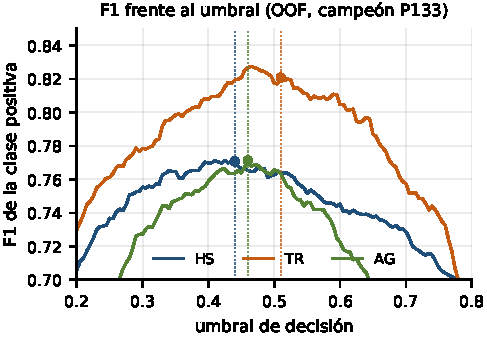
\includegraphics[width=\columnwidth]{fig_umbrales.pdf}
\caption{$F_1$ por etiqueta en función del umbral de decisión (OOF,
campeón P133). Las líneas verticales punteadas marcan los umbrales
congelados; los puntos, el valor que producen. Las mesetas son amplias, lo
que hace que el umbral exacto no sea crítico.}
\label{fig:umbrales}
\end{figure}

\subsection{Análisis de error}

La Tabla~\ref{tab:error} desglosa la matriz de confusión y el desempeño por
longitud. La Figura~\ref{fig:confusion} muestra las matrices de confusión
resultantes. De las tres columnas, TR obtiene el mayor $F_1$ (0.8207): el umbral
alto y el
ancla de positivos compensan su menor prevalencia. HS y AG quedan en 0.7707 y
0.7713, con 175 y 126 falsos positivos y 132 falsos negativos cada una. El
patrón por longitud es el hallazgo más claro: los tuits cortos alcanzan
0.8824, los medios 0.7544 y los largos 0.6306. La caída no es solo de
vocabulario: los textos largos contienen más contexto, más ironía y más
discurso citado, y el modelo lineal, que decide por suma de indicios, pierde
precisión cuando el contexto cambia el signo de una palabra.

\begin{table}[t]
\centering
\caption{Análisis de error del campeón. Arriba: matriz de confusión por
etiqueta (OOF). Abajo: $F_1$ por franja de longitud; los cortes son los
terciles de 70 y 118 caracteres.}
\label{tab:error}
\small
\begin{tabular}{lrrrrr}
\toprule
Etiqueta & TP & FP & FN & TN & $F_1$ \\
\midrule
HS & 516 & 175 & 132 & 660 & 0.7707 \\
TR & 364 & 78 & 81 & 960 & 0.8207 \\
AG & 435 & 126 & 132 & 790 & 0.7713 \\
\midrule
Franja & $n$ & Macro & HS & TR & AG \\
\midrule
Corta ($\le 70$) & 504 & 0.8824 & 0.8633 & 0.9000 & 0.8840 \\
Media ($71$--$118$) & 488 & 0.7544 & 0.7560 & 0.7742 & 0.7331 \\
Larga ($>118$) & 491 & 0.6306 & 0.6466 & 0.6250 & 0.6202 \\
\bottomrule
\end{tabular}
\end{table}

\begin{figure*}[t]
\centering
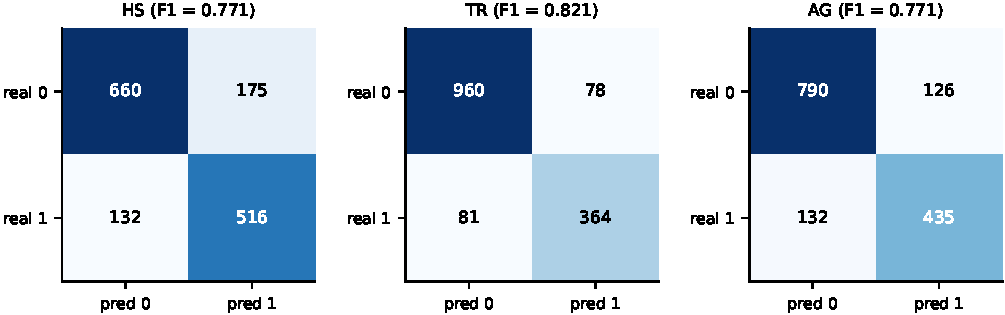
\includegraphics[width=\textwidth]{fig_confusion.pdf}
\caption{Matrices de confusión del campeón P133 sobre las predicciones OOF
de la partición canónica. La asimetría entre falsos positivos y falsos
negativos es distinta por etiqueta: HS sobrerrepresenta positivos, AG presenta
un leve sesgo hacia falsos negativos y TR está equilibrada (78/81).}
\label{fig:confusion}
\end{figure*}

El análisis por rebanadas de la fase inicial (sobre las 1\,731 filas y el
modelo V03) identifica las regiones más débiles: los tuits con hashtag
($F_1=0.586$), con pregunta (0.633), con referencia colectiva (0.639), el
cuartil superior de longitud (0.645) y los que no tienen mención (0.697). El
45.5\,\% de los falsos negativos de AG contiene una referencia colectiva,
frente al 13.9\,\% de los verdaderos positivos: la agresividad que se escapa
es, sobre todo, contra grupos. El régimen de respuesta con mención inicial
alcanza $F_1=0.876$, mientras que el régimen de noticia o atribución se queda
en 0.702. Estas cifras fijan el techo práctico del enfoque y orientan el
trabajo futuro.

Los errores residuales se agrupan en cuatro patrones. Primero, falsos
positivos léxicos: palabras vulgares en contextos inocentes (mascotas,
canciones, elogios, bromas entre amigos). Segundo, falsos negativos de odio
implícito: deshumanización o exclusión sin insulto del léxico vigilado.
Tercero, desacuerdos de anotación en TR, sobre todo cuando la definición de
la competencia y la de HatEval difieren. Cuarto, discurso citado o narrativo:
el tuit reproduce un insulto ajeno y el modelo lo atribuye al autor. Los
ejemplos se presentan enmascarados en el cuaderno para no reproducir el
contenido ofensivo. La consecuencia práctica es que buena parte del error
restante no es un problema de capacidad del modelo, sino de ambigüedad
semántica y de definición de la etiqueta.

\subsection{Validez externa y riesgo de sobreajuste al leaderboard}

La lectura honesta de los resultados exige separar dos cosas. El modelo base
se validó con particiones agrupadas, bootstrap y McNemar; su mejora sobre V03
es la parte que generalizaría a datos nuevos. La capa de pares compensados no
se validó así: sus reglas se diseñaron para textos concretos del test, con
cero coincidencias en entrenamiento, y se aceptaron o rechazaron con el
leaderboard público. Es una forma de adaptación al test, legítima dentro de
las reglas de la competencia, pero distinta de la generalización.

El riesgo es real. Con 47 envíos de modelos al leaderboard (más la sonda de
plantilla; 25 de esta serie) y un
leaderboard público fijo, la búsqueda adaptativa puede encontrar reglas que
mejoran esa muestra y no el conjunto privado. La incertidumbre marginal de la
métrica es apreciable: el error estándar bootstrap agrupado de la $F_1$ del
campeón en desarrollo es 0.0117; escalado al tamaño del test (1\,154), del
orden de 0.013. Las diferencias de 0.001--0.005 solo son interpretables porque
son pareadas y porque cada envío cambia un lote contable. La Figura~\ref{fig:bootstrap} resume las mejoras
locales y el desempeño por franja de longitud. La literatura sobre
holdouts reutilizables advierte que la adaptación repetida al mismo conjunto
puede inflar el resultado \cite{dwork2015reusable}. Varias salvaguardas
reducen el riesgo: los lotes preservan el número de positivos por columna, las
firmas léxicas son específicas, cada envío se audita antes de subirse y la
decisión se registra con su delta. Aun así, no eliminan el riesgo. El
leaderboard privado es la prueba final y, a la fecha de este informe, no se
conoce.

La consecuencia para el artículo es que el 0.81447 no debe leerse como una
estimación insesgada de la $F_1$ en población. Es el resultado de un sistema
en una competencia, con una capa de decisión adaptada al test. La estimación
limpia es la del modelo base: 0.787582 OOF, con IC95 para la mejora sobre
V03. Ambas cifras son ciertas; miden cosas distintas. Presentarlas separadas
es más informativo que quedarse con la más alta.

\subsection{Comparación con la literatura y límites}

Los sistemas clásicos de HatEval combinaron rasgos lingüísticos, n-gramas y
modelos lineales o neuronales, y muchos quedaron en el rango de 0.70--0.80 de
$F_1$ en español \cite{basile2019hateval,argotavega2019mineriaunam,ninaalcocer2019haterecognizer,pereirakohatsu2019haternet}.
Nuestro modelo base es coherente con esa familia y añade una ingeniería de
representación y decisión que lo lleva a la parte alta del rango, aunque la
comparación entre corpus no es directa. Los
transformers habrían sido la alternativa natural, pero estaban prohibidos; la
comparación directa con ellos no es posible en este contexto
\cite{plazadelarco2021comparing}. La capa de pares compensados es ortogonal
al modelo: podría aplicarse a cualquier base, siempre que se acepte su costo
de adaptación al test.

Los límites son claros. El corpus es pequeño (1\,731 filas), de un solo
idioma, normalizado a ASCII y con ruido de anotación; los near-duplicados se
mitigan con grupos, pero no desaparecen; la definición de TR es ambigua; y
la selección de 25 candidatos en el leaderboard introduce un sesgo de
selección que el bootstrap local no captura. No hubo validación externa ni
evaluación prospectiva. Estas limitaciones no invalidan el resultado, pero
acotan su alcance: es un sistema de competencia, reproducible y auditado, no
un clasificador listo para producción.

\begin{figure*}[t]
\centering
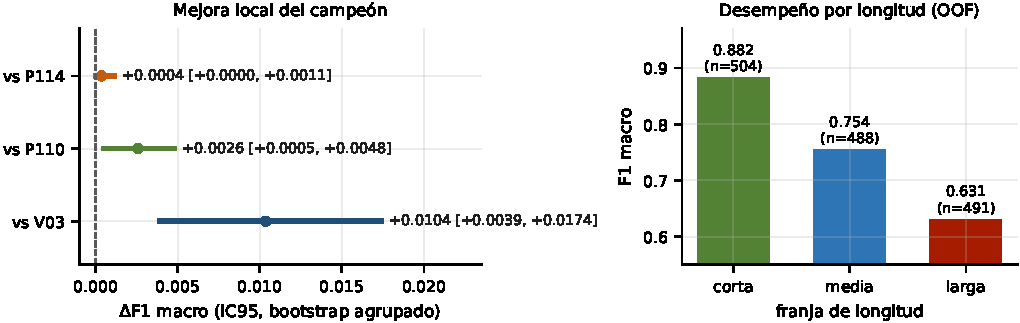
\includegraphics[width=\textwidth]{fig_bootstrap.pdf}
\caption{Izquierda: mejora local del campeón frente a V03, P110 y P114, con
IC95 por bootstrap agrupado. Derecha: $F_1$ macro por franja de longitud; la
caída en los textos largos es el principal frente de mejora.}
\label{fig:bootstrap}
\end{figure*}
